\documentclass{article}
\usepackage{graphicx} % Required for inserting images
\usepackage{listings}
\usepackage{hyperref}
\usepackage{float}
\usepackage{amsmath}
\usepackage{amssymb}
\usepackage{stmaryrd}
\usepackage{xcolor}
\usepackage[skip=10pt plus1pt]{parskip}
\usepackage{mathtools}

\hypersetup{
    colorlinks,
    linkcolor={red!50!black},
    citecolor={blue!50!black},
    urlcolor={blue!80!black}
}

\lstset{
  numbers=left,
  stepnumber=1,    
  firstnumber=0,
  numberfirstline=true,
  frame=single,
  mathescape
}

\newlength{\mylen}
\setbox1=\hbox{$\bullet$}\setbox2=\hbox{\tiny$\bullet$}
\setlength{\mylen}{\dimexpr0.5\ht1-0.5\ht2}
\renewcommand\labelitemi{\raisebox{\mylen}{\tiny$\bullet$}}

\setcounter{secnumdepth}{1}

\title{ITCS Notes}
\author{Christopher Dalziel}
\date{November-December 2023}

\setlength \parindent{0pt}
\setcounter{section}{-1}

\begin{document}

\maketitle

\tableofcontents\label{table-of-contents}

\newpage

\section{Introduction}
Hello! These are my notes for ITCS, which I hope will be useful to you if you're reading this.

These notes are adapted from the \href{https://www.inf.ed.ac.uk/teaching/courses/itcs/lectures.html}{excellent slides} provided by Dr. Liam O'Connor. Not all proofs are contained here, so if there's something that seems to be missing do check the slides!

I've added a definitions section, which mostly contains definitions which weren't in the course that are assumed knowledge from courses like DMP. Those definitions which were in the course but I've moved from the main body of the notes are the ones which I either felt stood well on their own (the note on \hyperref[tm]{Turing Machines} for example) or were not critical to understanding a general section of notes (e.g. \hyperref[parse-trees]{parse trees})

As with my CSEC notes there are \hyperref[table-of-contents]{highlighted sections of text} which act as links to different sections of the document - something I find particularly useful for this course!

I do hope these notes are useful to you, I've had good reviews on the CSEC ones - regardless, good luck with the exam!

\newpage

\section{Finite Automata}\label{finite-automata}
A finite automaton takes a string as input and replies "yes" or "no". If an automaton $A$ replies "yes" on a string $S$ we say $A$ "accepts" $S$.

A string $S$ is a possibly empty sequence of symbols from an alphabet $\Sigma$.

The language of a finite automaton $A$, written $\mathcal{L}(A)$ is the set of strings for which $A$ accepts.

\subsection{Deterministic Finite Automata}\label{dfa}
A deterministic finite automaton (DFA) is a quintuple $(Q, \Sigma, q_0, \delta, F)$ where:
\begin{itemize}
    \item $Q$ is a finite set of states
    \item $\Sigma$ is an alphabet
    \item $q_0 \in Q$ is the initial state
    \item $\delta : Q \times \Sigma \to Q$ is the transition function
    \item $F \subseteq Q$ is the set of final states
\end{itemize}

A DFA accepts a string $w \in \Sigma^*$ iff $\delta^*(q_0, w) \in F$, where $\delta^*$ is $\delta$ applied successively for each symbol in $w$. The language of a DFA $A$ is the set of all strings accepted by $A$, $\mathcal{L}(A) \subseteq \Sigma^*$ is the set of all strings accepted by $A$.

\begin{figure}[H]
    \centering
    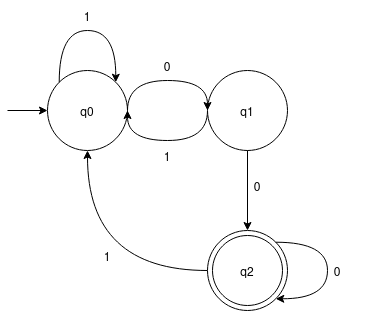
\includegraphics[scale=0.5]{images/dfa.png}
    \caption{Example of a DFA}
    \label{fig:dfa}
\end{figure}

The following pseudocode may help explain $\delta^*$ if the above is confusing:
\begin{lstlisting}[language=Python]
define d*(q_0: State, w: String) -> Boolean {
    state = q_0;
    
    for char in w {
        state = d(state, char);
    }
    
    return state in F;
}
\end{lstlisting}

In a DFA, the transition function is a \hyperref[total-partial]{total} function which gives exactly one next state for each input symbol. This means it is \hyperref[deterministic]{deterministic}.

If $\delta$ were partial we could express a total equivalent using less information - any partial DFA could be a total one.

\begin{figure}[H]
    \centering
    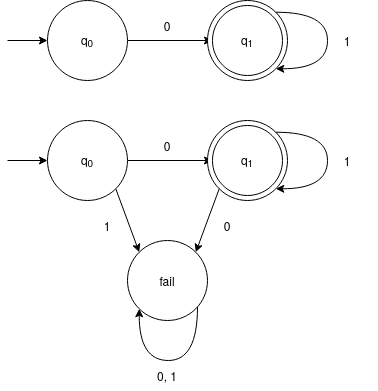
\includegraphics[scale=0.5]{images/partial-dfa.png}
    \caption{Partial DFA (top) and an equivalent total DFA (bottom)}
    \label{fig:partial-dfa}
\end{figure}

\subsection{Non-Deterministic Finite Automata}\label{nfa}
Non-determinism would mean that $\delta$ can return more than one successor state, it instead returns a set of possible states - no states is an empty set.

Non-deterministic finite automata (NFA) are \hyperref[angel-devil]{angelically} non-deterministic. An NFA is a quintuple $(Q, \Sigma, q_0, \delta, F)$ where:
\begin{itemize}
    \item $Q$ is a finite set of states
    \item $\Sigma$ is an alphabet
    \item $q_0 \in Q$ is the initial state
    \item $\delta : Q \times \Sigma \to \mathcal{P}(Q)$ is the transition function
    \item $F \subseteq Q$ is the set of final states
\end{itemize}

The only difference between the definition of a DFA and that of an NFA is that in an NFA $\delta$ returns an element from the \hyperref[power-set]{power set} of $Q$, $\mathcal{P}(Q)$.

Adding non-determinism doesn't change "expressivity". Given an NFA $A$ there is an equivalent DFA $D$ such that $\mathcal{L}(D)=\mathcal{L}(A)$ and vice versa.

\textbf{Proof}:
NFA $\to$ DFA: A DFA is already an NFA, one where the transition function always returns a singleton set.

DFA $\to$ NFA: This is harder, and we use the subset construction.

\subsubsection{Subset Construction}\label{subset-construction}
For an NFA $A$, the corresponding DFA $D$ tracks the set of states that $A$ could possibly be in, giving the string read so far. So each state of $D$ is a set of states from $A$.

Given an NFA $(Q_A, \Sigma, q_0, \delta_A, F_A)$, we can construct a DFA $(\mathcal{P}(Q_A), \Sigma, \{q_0\}, \delta_D, F_D)$ where:
\[\delta_D(S,a)=\bigcup_{q \in S} \delta_A(q, a) \text{ for each }S \subseteq Q\]
and:
\[F_D=\{S \subseteq Q \:|\: S \cap F_A \neq \emptyset\}\]

A subset construction involves making a DFA where the states are all possible combinations of states that the original NFA can be in.

\begin{figure}[H]
    \centering
    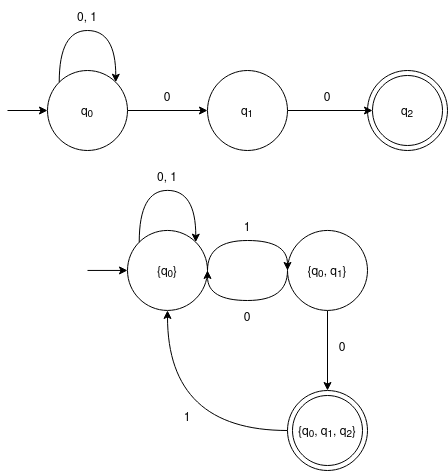
\includegraphics[scale=0.5]{images/subset-construction.png}
    \caption{An example of an equivalent DFA and NFA}
    \label{fig:subset-construction}
\end{figure}

\subsubsection{$\epsilon$-NFA}\label{epsilon-transitions}
If we allow non-deterministic state changes that don't consume any input symbols. We label silent moves using $\epsilon$ - meaning the empty string.

We define the $\epsilon$-closure $E(q)$ of a state $q$ as the set of all states reachable from $q$ by silent moves. That is, $E(q)$ is the least set satisfying:
 \begin{itemize}
     \item $q \in E(q)$
     \item For any $s \in E(q)$ we also have $\delta(s, \epsilon) \subseteq E(q)$
 \end{itemize}

 We also extend this to sets where $E(s) = \bigcup\limits_{q \in s}{E(q)}$

 These too are equal in expressive power to NFA and DFA.

\newpage

\section{Regular Languages}\label{regular-languages}
Any language which can be accepted by a finite automaton is called a regular language.

Regular languages are also those recognised by Regular Expressions.

\subsection{Regular Expressions}\label{regex}
Regular expressions exactly characterise the regular languages, just as finite automata do.

The following table shows the syntax and semantics (the meaning of the syntax) of a regular expression.

begin{table}[H]
    \begin{tabular}{l|ll}
    Syntax          & Semantics                                                                                       &                  \\ \hline
    $a$             & $\llbracket a \rrbracket = \{a\}$                                                               & $(a \in \Sigma)$ \\
    $\emptyset$     & $\llbracket \emptyset \rrbracket = \emptyset$                                                   &                  \\
    $\epsilon$      & $\llbracket \epsilon \rrbracket = \{\epsilon\}$                                                 &                  \\
    $R_1 \cup R_2$  & $\llbracket R_1 \cup R_2 \rrbracket = \llbracket R_1 \rrbracket \cup \llbracket R_2 \rrbracket$ &                  \\
    $R_1 \circ R_2$ & $\llbracket R_1 \circ R_2 \rrbracket = \llbracket R_1 \rrbracket \llbracket R_2 \rrbracket$     &                  \\
    $R^*$           & $\llbracket R^* \rrbracket = \llbracket R \rrbracket^*$                                         &                 
    \end{tabular}
    \centering
\end{table}

\textbf{Examples}:
At least one 0:
\[(0 \cup 1)^* 0 (0 \cup 1)^*\]

At least one 1 and at least one 0:
\[((0 \cup 1)^*01(0 \cup 1)^*) \cup ((0 \cup 1)^*10(0 \cup 1)^*)\]

\subsection{Generalised NFA}\label{gnfa}
A generalised NFA is an NFA where transitions have regular expressions instead of symbols, there is only one unique final state, and the transition relation is full, except that the initial state has no ingoing transitions and the final state no outgoing ones.

The process to do this is as follows:
\begin{enumerate}
    \item Add a new start state, connected via $\epsilon$ transitions to the old one
    \item Add a new final state, connected via $\epsilon$ transitions to all old final states
    \item If two states $q_0$ and $q_1$ have two transitions between them $q_0 \xrightarrow[]{a} q_1$ and $q_0 \xrightarrow[]{b} q_1$, replace them with $q_0 \xrightarrow[]{a \cup b} q_1$
    \item Introduce $\emptyset$-labelled transitions where needed to make the transition relation full
\end{enumerate}

By eliminating each of the inner states of a GNFA one by one, you can get a GNFA with a start and final state connected by a single transition between them. The label on that transition is the regular expression that characterises the original GNFA.

\newpage

\section{Beyond Regular Languages}\label{non-regular-languages}
Most languages are not \hyperref[regular-languages]{regular}, programming languages for example are mostly non-regular.

Determining matching parentheses is non-regular.
\[ L_{()} = \{(^n \: )^n \:|\: n \in \mathbb{N}\} \]

Doing this would require counting the number of opening brackets as a regular string - an unbounded natural number, requiring unbounded memory and resulting in non-finite states.

This breaks the definition of a \hyperref[finite-automata]{Finite Automaton} - meaning it cannot be represented by one, and so mustn't be a regular language.

To determine if a language is regular or not we have two methods: the Pumping Lemma and the Myhill-Nerode Theorem.

\subsection{The Pumping Lemma}\label{pumping-lemma}
If a DFA with $k$ states accepts a word of length greater than $k$, we know that the DFA must have visited one of its states \hyperref[pigeonhole-principle]{more than once} - the DFA must have a loop.

Therefore if we go through the loop any number of times, the DFA will accept those words too. We call this "pumping".

If $L \subseteq \Sigma^*$ is regular then there's a pumping length $p \in \mathbb{N}$ such that for any $w \in L$ where $|w| \geq p$, we may split $w$ into three pieces $w=xyz$ satisfying three conditions:
\begin{itemize}
    \item $xy^iz \; \forall i \in \mathbb{N}$
    \item $|y| > 0$, and
    \item $|xy| \leq p$
\end{itemize}

Because we know that this is true for all regular languages, the contrapositive statement - that if we can't pump a language it isn't regular - must also be true.

Importantly, the opposite is not true. Meaning that not all pumpable languages are regular.

\subsection{The Myhill-Nerode Theorem}\label{myhill-nerode}
Let $L \subseteq \Sigma^*$ and $x,y \in \Sigma^*$, if there exists a suffix string $z$ such that $xz \in L$ but $yz \not\in L$ or vice versa, then $x$ and $y$ are distinguishable by $L$.

If $x$ and $y$ are not distinguishable by $L$, then we say $x \equiv_L y$ - this is an \hyperref[equivalence-relation]{equivalence relation}.

A language $L$ is regular iff the number of \hyperref[equivalence-class]{equivalence classes} using this relation $\equiv_L$ is finite. If there were not a finite number of classes there would need to be an infinite number of states in the DFA.

To show a language is non-regular then, we can show that it has infinite equivalence classes - that is, we find an infinite sequence $u_0u_1u_2\dots$ of strings such that for any $i, j$ (where $i \neq j$) there is a string $w_{ij}$ such that $u_iw_{ij}\in L$ but $u_jw_{ij}\not \in L$ or vice-versa.

For the matching brackets example we can choose $u_i = (^i$ and $w_{ij}=)^i$.

\newpage

\section{Context-free Languages}\label{cfl}
By adding recursion to regular expressions we can begin to recognise some non-regular languages.

All regular languages are context free.

A language is context-free iff it is recognised by a \hyperref[cfg]{context-free grammar}.

\subsection{Context-free Grammars}\label{cfg}
A Context-free Grammar (CFG) is a 4-tuple $(N, \Sigma, P, S)$ where:
\begin{itemize}
    \item $N$ is a finite set of variables or non-terminals
    \item $\Sigma$ is a finite set of terminals
    \item $P \subseteq N \times (N \cup \Sigma)^*$ is a finite set of rules or productions.
    \begin{itemize}
        \item Typically productions are written $A \to aBc$
        \item Productions with common heads can be combined, $A \to a$ and $A \to Aa$ can be combined into $A \to a \:|\: Aa$
    \end{itemize}
    \item  $S \in N$ is the starting variable
\end{itemize}

We use $\alpha, \beta, \gamma$ to refer to sequences of terminals.

We make a derivation step $\alpha A \beta \Rightarrow_G \alpha \gamma \beta$ whenever ($A \to \gamma$) $\in P$; The language of a CFG $G$ is:
\[\mathcal{L}(G)=\{w \in \Sigma^* \:|\: S \Rightarrow_G^* w^*\}\]

Where $\Rightarrow_G^*$ is the \hyperref[reflexive]{reflexive}, \hyperref[transitive]{transitive}, \hyperref[closure]{closure} of $\Rightarrow_G$.

Context-free grammars are \hyperref[ambiguity]{ambiguous}. They are \hyperref[closure]{closed} under union, concatenation, and kleene star.


\subsection{Eliminating Ambiguity}
We want to eliminate \hyperref[ambiguity]{ambiguity} in \hyperref[cfg]{context-free grammars} while still accepting all the same strings.

This can be done for our language of \hyperref[regex]{regular expressions}:
\begin{itemize}
    \item First defining atomic expressions: $A \to (S) \:|\:\emptyset \:|\:\epsilon \: | \: a \: | \: b$
    \item Then ones which use \hyperref[kleene-star]{Klene Star}: $K \to A \:|\: A^*$
    \item Then ones which may use left-associative composition: $C \to K \:|\: C \circ K$
    \item Finally expressions which use unions: $S \to C \:|\: S \cup C$
\end{itemize}

The order of operations here is therefore bottom to top; unions come before compositions come before kleene star etc.

\subsection{Push-down Automata}\label{pda}
Push-down automata are to \hyperref[cfg]{context-free grammars} what \hyperref[finite-automata]{finite automata} are to \hyperref[regex]{regular expressions}.\\

They are implementationally identical to  $\epsilon$-NFA with one addition, a stack. The recursive element of CFGs is implemented using a standard last-in-first-out stack.

Transitions in a push-down automata take the form $x, y \to z$, which is read as "consume the input $x$, popping $y$ off the stack, and push $z$ onto the stack". We can allow actions that don't consume, pop, or push by setting $x, y$, or $z$ to $\epsilon$.

PDA operate on an input alphabet $\Sigma$, but their stack has its own "stack alphabet": $\Gamma = \Sigma \cup \{\bullet\}$. This bullet ($\bullet$) character is used for bookkeeping, usually as a way of determining when we've reached the bottom of the stack.


\begin{figure}[H]
    \centering
    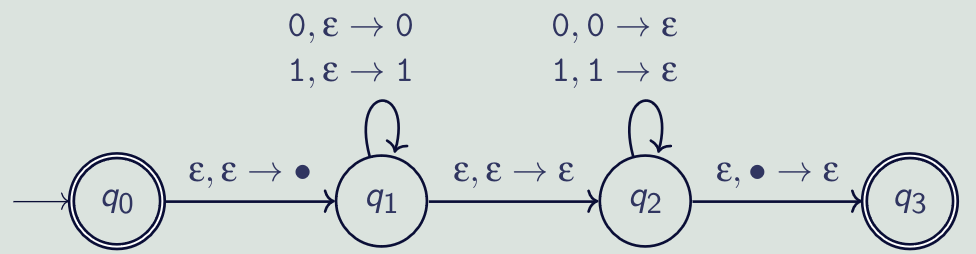
\includegraphics[width=0.75\linewidth]{images/pda.png}
    \caption{A PDA for recognising even length palindromes on $\Sigma = \{0, 1\}$}
\end{figure}

Formally, a push-down automata is a 6-tuple ($Q, \Sigma, \Gamma, \delta, q_0, F$) where $Q, \Sigma$, and $\Gamma$ are all finite sets. 

$\Gamma$ is the stack alphabet and $\delta$ now may take a stack symbol as input or return one as output.
\[\delta : Q \times \Sigma_{\epsilon} \times \Gamma_{\epsilon} \to \mathcal{P}(Q \times \Gamma_{\epsilon})\]

A string $w$ is accepted by a PDA if it ends in a final state, i.e. $\delta^*(q_0, w, \epsilon)$ gives a state $q$ and a stack $\gamma$ such that $q \in F$.

Any language that is recognised by a push-down automata is context free.

\subsubsection{CFG to PDA}
The upper loop on $q_1$ is added for every terminal $a$ in the CFG. The lower loop on $q_1$ is shorthand for a looping sequence of states added for each production $A \to w$ that builds up $w$ on the stack one symbol at a time.

\begin{figure}[H]
    \centering
    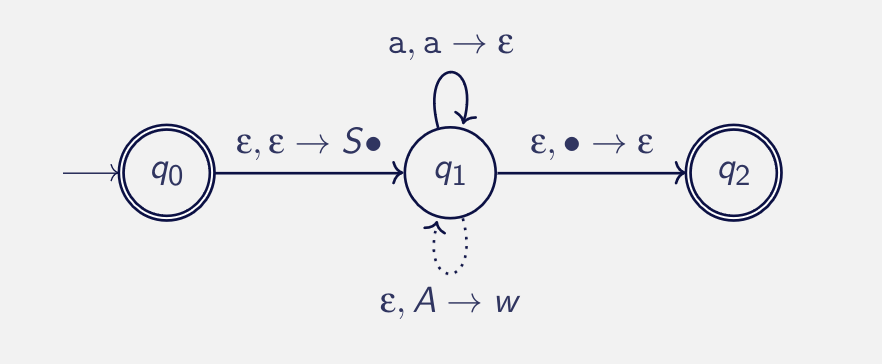
\includegraphics[width=0.75\linewidth]{images/cfg-to-pda.png}
    \caption{The general form of converting a CFG to a PDA}
\end{figure}


\subsubsection{PDA to CFG}
Firstly we ensure that the PDA has only one accept state, empties its stack before terminating, and has only transitions that either push or pop a symbol (but not transitions that do both or neither).

Given such a PDA $P=(Q, \Sigma, \Gamma, \delta, q_0, F)$ we provide a CFG $(V, \Sigma, R, S)$ with $V$ containing a non-terminal $A_{pq}$ for every pair of states $(p,q) \in Q \times Q$.

The non-terminal $A_{pq}$ generates all strings that go from $p$ with an empty stack to $q$ with an empty stack. Then $S$ is just $A_{q_0q_{accept}}$.

$R$ consists of:
\begin{itemize}
    \item $A_{pq} \to aA_{rs}b$ if $p \xrightarrow[]{a,\epsilon \to t}r$ and $s \xrightarrow[]{b, t, \to \epsilon}q$ (for intermediate states $r, s$ and stack symbol $t$
    \item $A_{pq} \to A_{pr}A_{rq}$ for all intermediate states $r$
    \item $A_{pp} \to \epsilon$
\end{itemize}

\subsection{Pumping for CFLs}
Supposing a \hyperref[cfg]{CFG} has $n$ non-terminals, and the parse tree has a height $k > n$, we know that some non-terminal state $v$ \hyperref[pigeonhole-principle]{must appear as its own descendant} in the tree.

Unlike when \hyperref[pumping-lemma]{pumping for regular languages}, we can pump up or down the parse tree when pumping for context-free languages.

We can pump down by cutting the tree at a higher occurrence of $V$ and replacing it with the sub-tree at the lower occurrence of $V$.

We can pump up by cutting away the lower occurence of $V$ instead, and replacing it with a fresh copy of the higher occurence.

If a language $L$ is context-free, then there exists a pumping length $p \in \mathbb{N}$ such that if $w \in L$ with $|w| \geq p$ then $w$ may be split into five pieces $w = uvxyz$ such that:
\begin{enumerate}
    \item $uv^ixy^iz \in L \; \forall i \in \mathbb{N}$
    \item $|vy| > 0$ and
    \item $|vxy| \leq p$
\end{enumerate}

The general rule of thumb should be to pick a string $w$ that allows as few cases for partitions of $w = uvxyz$ as possible

\subsection{Chomsky Grammars}\label{context-sensitive}
\hyperref[cfg]{Context-free grammars} are a special case of Chomsky Grammars. Chomsky grammars are similar to CFG, except that the left-hand side of a production may be any string that includes at least one non-terminal.

\[S \to abc \:|\: aAbc\]
\[Ab \to bA\]
\[\vdots\]

Such a grammar is called "context-sensitive".

\subsection{The Chomsky Hierarchy}
A grammar $G = (N, \Sigma, P, S)$ is of type:
\begin{enumerate}
    \setcounter{enumi}{-1}
    \item (or computably enumarable/turing recognisable) in the general case.
    \item (or \hyperref[context-sensitive]{context-sensitive}) if $|\alpha| \leq |\beta|$ for all productions $\alpha \to \beta$, except we also allow $S \to \epsilon$ if $S$ does not occur on the right hand side of any rule.
    \item (or \hyperref[cfg]{context-free}) if all productions are of the form $A \to \alpha$.
    \item (or right-linear/\hyperref[regular-languages]{regular languages}) if all productions are of the form $A \to w$ or $A \to wB$ where $w \in \Sigma$ and $B \in N$.
\end{enumerate}

\newpage

\section{Algorithms for Languages}
\subsubsection{Emptiness for Regular Languages}
Can we write a program to determine if a given \hyperref[regular-languages]{regular language} is empty?

Given a finite-automaton this is an instance of graph reach-ability, so we can use a depth-first search.

\subsubsection{Emptiness for Context-free Languages}
Can we write a program to determine if a given \hyperref[cfg]{context-free language} is empty?

Given a CFG for our language, we can perform the following process:
\begin{enumerate}
    \item Mark the terminals and $\epsilon$ as generating
    \item Mark all non-terminals which have a production with only generating symbols in their right hand side as generating
    \item Repeat until nothing new is marked
    \item Check if $S$ is marked as generating or not
\end{enumerate}

\subsubsection{Equivalence of DFA}
Is it possible to write a program to determine if two \hyperref[dfa]{discrete finite automata} are equivalent?

Given two DFA for $L_1$ and $L_2$, we can use our standard constructions to produce a DFA of the symmetric set difference:
\[(L_1 \cap \overline L_2) \cup (L_2 \cap \overline L_1)\]

\newpage

\section{Register Machines}\label{rm}
A register machine, or RM, consists of:
\begin{itemize}
    \item a fixed number $m$ of registers $R_0 \dots R_{m-1}$, which each hold a natural number
    \item a fixed program $P$ which is a sequence of $n$ instructions $I_0 \dots I_{n-1}$
\end{itemize}

Each instruction is one of the following:
\begin{itemize}
    \item \texttt{INC(i)}: which increments the register $R_i$ by one
    \item \texttt{DECJZ(i, j)}: which decrements register $R_i$ unless $R_i = 0$ in which case it jumps to instruction $I_j$
\end{itemize}

With RMs we \hyperref[universality]{can compute anything} that another computer can compute. 

Their major flaw is that at present they're tedious and cumbersome to work with. We can fix this with "macros", which make it more similar to a real world assembly language.

This includes new instructions, which can make simple tasks like addition simple again, and including symbolic labels for jumps.

Our macros are allowed to access special negative-indexed registers which we can guarantee won't be used by normal programs - this is entirely for convenience and does not give us any more exclusivity.

\subsubsection{Example Macros for RMs}
Goto $I_j$ using $R_{-1}$ as temp (\texttt{GOTO(j)}):
\begin{lstlisting}
        DECJZ -1, j
\end{lstlisting}

Clear $R_i$ (\texttt{CLEAR(i)}):
\begin{lstlisting}
        DECJZ i, 2
        GOTO 0
\end{lstlisting}

Copy $R_i$ to $R_j$ using $R_{-2}$ as temp (\texttt{COPY(i, j)}:
\begin{lstlisting}
        CLEAR $R_j$
loop_1: DECJZ i, loop_2
        INC R_j
        INC R_{-2}
        GOTO loop_1
loop_2: DECJZ R_{-2}, end
        INC R_i
        GOTO loop_2
end:
\end{lstlisting}

\subsubsection{How many registers?}
So far we've made the assumption that we have as many \hyperref[rm]{RM} registers as we need, but how many do we actually need?

We can use a \hyperref[pairing-function]{pairing function} and a corresponding unpairing function to pack every value we need into a single register - meaning we only need as many registers as the pairing function requires and a single user register. This turns out to give us that two registers is enough.

\subsection{Universality}\label{universality}\label{encoding}
A model of computation is universal if it can simulate any other model of computation. To simulate a machine we need a machine which given some encoding of a machine $M$ (written $\ulcorner M \urcorner$) as input will produce the correct result of running $M$ as output.

To start proving a model of computation is universal it is generally useful to prove that it can simulate itself.

For a given \hyperref[rm]{register machines} $M$, making an encoding involves using a \hyperref[pairing-function]{pairing function} to pack our instructions and registers into a single value $\ulcorner M \urcorner$.

\begin{equation}
\begin{aligned}
    \ulcorner INC(i) \urcorner &= \langle 0, i \rangle \\
    \ulcorner DECJZ(i, j) \urcorner &= \langle 1, i, j \rangle \\
    \ulcorner P \urcorner &= \langle \ulcorner I_0 \urcorner, \dots, \ulcorner I_{n-1} \urcorner \rangle \\
    \ulcorner R \urcorner &= \langle R_0, \dots, R_{m-1} \rangle \\
    \ulcorner M \urcorner &= \langle \ulcorner P \urcorner, \ulcorner R \urcorner \rangle
\end{aligned}
\end{equation}

\subsubsection{The Church-Turing Thesis}
The Church-Turing thesis states that any problem is computable by any model of computation iff it is computable by a \hyperref[tm]{Turing Machine}.

For our purposes this matters for \hyperref[rm]{RMs}, \hyperref[tm]{TMs}, and \hyperref[lambda-calculus]{$\lambda$-calculus}.

Other examples are combinator calculus, general recursive functions, pointer machines, counter machines, cellular automata, queue automata, enzyme-based DNA computers, Minecraft, \href{https://arxiv.org/pdf/1904.09828.pdf}{Magic the Gathering} (highly recomend this paper), and others.

\newpage

\section{Decidability}
\subsection{Problems with no Algorithm}
While the above problems are all computable, this is not always the case. The questions asked, i.e. "can we determine $x$?", are not always something we can answer using a program - if this is the case then that problem is considered \hyperref[undecidable]{undecidable}.

Many such problems exist for \hyperref[cfl]{Context-free Languages}:
\begin{itemize}
    \item Are two CFG equivalent?
    \item Is a given CFG \hyperref[ambiguity]{ambiguous}?
    \item Is there a way to make a given CFG unambiguous?
    \item Is the intersection of two CFLs empty?
    \item Does a CFG generate all strings $\Sigma^*$?
    \item $\dots$
\end{itemize}

\subsection{The Halting Problem}\label{halting}
Given a \hyperref[rm]{register machine} \hyperref[encoding]{encoding} can we write a program to determine if the simulated machine will halt or not?

If we suppose $H$ is such a register machine, which takes a machine encoding $\ulcorner M \urcorner$ in $R_0$ and halts with $1$ if $M$ halts and halts with $0$ if $M$ doesn't halt.

We can construct a new machine $L = (P_L, R_0, \dots)$ which, given a program $\ulcorner P \urcorner$ runs $H$ on the program with itself as input, the machine $(P, \ulcorner P \urcorner)$ and loops if it halts.

If we run $L$ on $P_L$ itself we get a problem. If $L$ halts on $\ulcorner P_L \urcorner$ that means $H$ says $(P_L, \ulcorner P_L \urcorner)$. If $L$ loops on $\ulcorner P_L \urcorner$ that means that $H$ says $(P_L, \ulcorner P_L \urcorner)$ halts.

This is a contradiction!

The halting problem proves that there are some programs which cannot be decided by register machines. What about other machines?

\newpage

\section{Undecidability}\label{undecidable}
The existence of the \hyperref[halting]{halting problem} means we know there can be problems which are not decidable. We can use a counting argument to point out that there are uncountably many languages and RMs are enumerable, so there are languages which are not decided (or even recognised) by any RM.

There are many \hyperref[undecidable-problems]{undecidable problems} - but how do we show that a problem is undecidable?

\subsection{Reductions}
A reduction is a transformation from one problem to another. To prove that a problem $P_2$ is hard, show that there is an easy reduction from a known hard problem $P_1$ to $P_2$.

To prove that a problem $P_2$ is undecidable, show that there is a computable reduction from a known undecidable $P_1$ to $P_2$. The direction here matters - it tells us nothing to know that there's an easy way to make an easy problem difficult!

If it is a well known fact that Hyunwoo cannot lift a car, we can prove that Hyunwoo cannot lift a loaded truck by making the following reduction: If we suppose he could lift the loaded truck, then we could have him lift the car by putting it in the loaded truck - but we know he cannot lift a car.

\subsubsection{Mapping Reductions}\label{mapping-reduction}
A mapping reduction (or a many-to-one reduction) from $P_1$ to $P_2$ is a \hyperref[turing-transducer]{Turing transducer} $f$ such that $d \in Q_1$ iff $f(d) \in Q_2$.

If $A$ is mapping reducible to $B$, and $A$ is undecidable, then $B$ is undecidable.

\subsubsection{Turing Reductions}\label{turing-reduction}
A Turing reduction from $P_1$ to $P_2$ is an \hyperref[rm]{RM}/\hyperref[tm]{TM} equipped with an oracle for $P_2$ which solves $P_1$.

Decidability results carry across during Turing reductions as with \hyperref[mapping-reduction]{mapping reductions}, but mapping reductions make finer distinctions of computing power.


\subsection{Rice's Theorem}
All \hyperref[nontrivial]{nontrivial} \hyperref[semantic]{semantic} \hyperref[property]{properties} are \hyperref[undecidable]{undecidable}.

Rice's theorem is useful for deciding properties like whether a language is empty, non-empty, regular, context-free etc.

It cannot be applied to questions like whether a TM has fewer than 7 states, a final state, a start state etc. These properties are of machines and not languages.

It also doesn't apply to questions like is a language a subset of $\Sigma^*$ or whether a language of a \hyperref[rm]{RM} is a language of a \hyperref[tm]{TM} - these are trivial properties!

The consequences of this is that we cannot write programs which answer non-trivial questions about the black-box behaviours of programs.

\newpage

\section{Computability}

\subsection{Computably Enumerable}
A set $S$ is called computably enumerable if the \hyperref[enumerable]{enumeration function} $f : \mathbb{N} \to S$ is \hyperref[computable]{computable}.

In terms of \hyperref[rm]{RM} and \hyperref[tm]{TM} we can think of enumeration as outputting an infinite list as it executes forever.

The \hyperref[halting]{halting problem} may be \hyperref[undecidable]{undecidable}, but is it computably enumerable? Yes! \hyperref[interleaving]{Interleaving} shows that $H$ is computably enumerable.

All semi-decidable problems are computably enumerable, and any computably enumerable problem is semi-decidable - being semi-decidable is the same as being computably enumerable.

To prove that a problem $P_2$ is not c.e. we show that there is a \hyperref[mapping-reduction]{mapping reduction} from a known not-c.e. problem $P_1$ to $P_2$. We must use mapping reductions, as $H$ is c.e. but $L$ is not - but $L$ is \hyperref[turing-reduction]{Turing reducible} to $H$ by flipping the answer.


\subsection{Complexity Measures}
When performing addition in a \hyperref[tm]{TM} we have a \hyperref[time-complexity]{time complexity} of $\mathcal{O}(\log n)$, where it is $\mathcal{O}(n)$ for \hyperref[rm]{RMs} - there's an exponential penalty for using a register machine!

Addition can be $\mathcal{O}(1)$ if we add dedicated \texttt{ADD(i, j)} and \texttt{SUB(i, j)} instructions - but this doesn't remove the inaccuracy it just makes it smaller.

Complexity is useful, but the measures are slightly bogus:
\begin{itemize}
    \item $\mathcal{O}(n)$ is not always easy - if $n$ is massive for example
    \item $\Omega(2^n)$ isn't always hard - there are problems much worse than this that are still solvable for real examples
    \item $\mathcal{O}(n^{10})$ and $\Omega(n^{10})$ seem extremely difficult, but a new model or algorithm could reduce that significantly
    \item Since we also ignore coefficients, we could have something like $f(n) \geq 10^{100} \log n$ which is slow but still only logarithmic - this isn't common enough to worry generally however.
\end{itemize}

\subsection{Complexity Classes}
Let $t:\mathbb{N} \to \mathbb{R}_{\geq 0}$. A time complexity class \textbf{TIME}$(t(n))$ is the collection of all problems that are decidable by a deterministic machine (\hyperref[rm]{RM}, \hyperref[tm]{TM} etc.) in $\mathcal{O}(t(n))$ time.

Given $A = \{0^i1^i \:|\: i \in \mathbb{N}\}$, a \hyperref[tm]{TM} can decide this in $\mathcal{O}(n^2)$, which means that $A \in$ \textbf{TIME}$(n^2)$.

We also define \textbf{NTIME}$(t(n))$ to be the collection of all problems decidable by a nondeterministic machine (\hyperref[nrm]{NRM}, NTM, etc.) in $\mathcal{O}(t(n))$.

\begin{figure}[H]
    \centering
    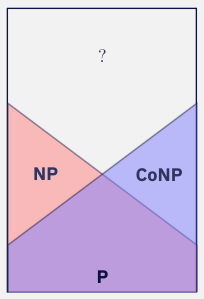
\includegraphics[width=0.25\linewidth]{images/basic-complexity-classes.png}
    \caption{The three basic complexity classes}
\end{figure}

\subsubsection{P: Polynomial Time}\label{P}
The polynomial complexity class \textbf{P} is the class of problems decidable with some deterministic polynomial time complexity.
\[\textbf{P} = \bigcup_{k \in \mathbb{N}} \textbf{TIME}(n^k)\]

Problems in \textbf{P} are called tractable. Any problem not in \textbf{P} is $\Omega(n^k)$ for every $k$.

The class itself is robust, reasonable changes to model don't change it and reasonable translations between problems preserves membership in \textbf{P}.

A polynomially-bounded \hyperref[rm]{RM} together with a polynomial ($n^k$ for some $k$, without loss of generality), such that given an input $w$ it will always halt after executing $|w|^k$ instructions. A problem $Q$ is in \textbf{P} iff it is computed by such a machine.

\subsubsection{NP: Nondeterministic-polynomial Time}\label{NP}
The polynomial complexity class \textbf{NP} is the class of problems decidable with some nondeterministic polynomial time complexity.
\[\textbf{NP} = \bigcup_{k \in \mathbb{N}} \textbf{NTIME}(n^k)\]

We don't know if every exponentially bounded problem is in \textbf{NP}, we think that it's probably not the case.

\subsubsection{CoNP}\label{CoNP}
We don't know if the class \hyperref[NP]{\textbf{NP}} is closed under complement. We cannot flip the result because the result of flipping in a \hyperref[nrm]{nondeterministic machine} involves turning it from angelic nondeterminism to demonic nondeterminism (otherwise known as co-nondeterminism) or vice versa.

\subsubsection{AP: Alternating Polynomial Time}\label{AP}
The class \textbf{AP} is the class of all problems decidable by an \hyperref[alternating-machine]{alternating machine} in polynomial time with no restriction on swapping quantifiers.

\textbf{AP} is known to be equal to \hyperref[PSPACE]{\textbf{PSPACE}}.

\subsubsection{PSPACE: Polynomial Space}\label{PSPACE}
An \hyperref[rm]{RM}/\hyperref[tm]{TM} is $f(n)$-space-bounded if it may use only $f(inputsize)$ space. For TMs this is the number of cells on the tape, where register machines uses bits in registers.


\subsection{Polynomial Reductions}\label{polynomial-reduction}
A polynomial reduction from $P_1 = (D_1, Q_1)$ to $P_2 = (D_2, Q_2)$ is a \textbf{P}-computable function $f : D_1 \to D_2$ such that $d \in Q_1$ iff $d \in Q_2$.

If $P_2$ is in \textbf{P}, then $P_1$ is in \textbf{P} straightforwardly. Therefore to prove a problem is not in \textbf{P} we can show that there is a polynomial reduction from a problem $P_2$ which \hyperref[NP]{isn't in \textbf{P}} to our problem $P_1$

A problem $P_1$ is polynomially reducible to $P_2$, written $P_1 \leq_P P_2$ if there is a polynomially-bounded reduction from $P_1$ to $P_2$.

\subsubsection{NP-Hard}\label{np-hard}
A problem $P$ is \textbf{NP}-Hard if for every $A \in$ \textbf{NP}, $A \leq_P P$.

That is, if a problem $P_1$ is \textbf{NP}-Hard and $P_1$ is \hyperref[polynomial-reduction]{polynomially reducible} to $P_2$, then $P_2$ is also \textbf{NP}-Hard.

We can use this fact to prove other problems are \textbf{NP}-Hard by showing a reduction from a known \textbf{NP}-hard problem.

\subsubsection{NP-Complete}\label{np-complete}
A problem is \textbf{NP}-Complete if it is both \hyperref[np-hard]{\textbf{NP}-Hard} and in \hyperref[np]{\textbf{NP}}.

\subsection{The Cook-Levin Theorem}
The Cook-Levin theorem states that the \hyperref[NP]{\textbf{NP}} problem \hyperref[sat]{SAT} is \hyperref[np-complete]{\textbf{NP}-Complete}.

The proof of this involves showing it is \textbf{NP} by nondeterministically guessing assignments and checking them in polynomial time, and then showing it's \textbf{NP}-Hard by reducing any \textbf{NP} problem to SAT.

\newpage

\section{The Polynomial Heirarchy}
\subsection{$\Sigma$s}
The set $\Sigma_1^P$ describes all problems which can be phrased as $\{y \:|\: \exists^P x \in \mathbb{N}.\: R(x,y)\}$, where $R$ is a \hyperref[P]{\textbf{P}}-decidable predicate and $\exists^P x \dots$ indicates that $x$ is of size polynomial in the size of $y$.

We can say that $x$ is a certificate showing which guesses can be made by our \hyperref[nrm]{NRM} giving an accepting run.

If a problem $Q \in \Sigma_1^P$ then $Q$ is \hyperref[NP]{\textbf{NP}}, because it is a problem for which we can verify the answer in polynomial time. If a problem $Q$ is in \textbf{NP} then $Q \in \Sigma_1^P$.

So, \textbf{NP} = $\Sigma_1^P$

\subsection{$\Pi$s}
The set $\Pi_1^P$ describes all problems that can be phrased as $\{y \:|\: \forall^P x \in \mathbb{N}. \: R(x,y)\}$, where $R$ is a \hyperref[P]{\textbf{P}}-decidable predicate and $\forall^P x \dots$ indicates that $x$ is of size polynomial in the size of $y$.

$\Pi_1^P = \overline{\Sigma_1^P}$, and $\Pi_1^P=$ \hyperref[CoNP]{\textbf{CoNP}}

\subsection{$\Delta$s}
There are two subtly conflicting definitions of $\Delta_1^P$:
\begin{enumerate}
    \item The set $\Delta_1^P$ describes the intersection of $\Sigma_1^P$ and $\Pi_1^P$
    \item The set $\Delta_1^P$ describes the set \hyperref[P]{\textbf{P}}
\end{enumerate}

\subsection{Moving Higher}
The next layer of the heirarchy goes as follows:
\begin{itemize}
    \item $\Sigma_2^P$ is all problems of the form $\{x \:|\: \exists^P y.\: \forall^P z.\: R(x,y,z)\}$
    \item $\Pi_2^P$ is all problems of the form $\{x \:|\: \forall^P y.\: \exists^P z.\: R(x,y,z)\}$
    \item $\Delta_2^P = \Sigma_2^P \cap \Pi_2^P$
\end{itemize}

We can also use \hyperref[oracle]{oracles} to get an alternate definition:
\begin{itemize}
    \item $\Delta_2^P$ is all problems that are \hyperref[decidable]{decidable} in \hyperref[P]{polynomial time} by some deterministic \hyperref[rm]{RM}/\hyperref[tm]{TM} with an $\mathcal{O}(1)$ oracle for some problem in $\Sigma_1^P$ (it is \textbf{P} with an $\mathcal{O}(1)$ oracle for \hyperref[NP]{\textbf{NP}})
    \item $\Sigma_2^P$ allows the TM/RM to be nondeterministic (it is \textbf{NP} with an $\mathcal{O}(1)$ oracle for \textbf{NP})
    \item $\Pi_2^P$ is \hyperref[CoNP]{\textbf{CoNP}} with an oracle for \textbf{NP}
\end{itemize}

In general for any $n>1$:
\begin{itemize}
    \item $\Delta_n^P$ is all problems decidable by a deterministic polynomially bounded TM/RM with an $\mathcal{O}(1)$ oracle for some problem in $\Sigma_{n-1}^P$.
    \item $\Sigma_n^P$ is all problems decidable by some nondeterministic polynomially bounded TM/RM with an $\mathcal{O}(1)$ oracle for some problem in $\Sigma_{n-1}^P$.
    \item $\Pi_n^P$ is all problems decidable by some co-nondeterministic polynomially bounded TM/RM with an $\mathcal{O}(1)$ oracle for some problem in $\Sigma_{n-1}^P$.
\end{itemize}

\subsubsection{Alternation}
Equivalently to the general definition given above, $\Sigma_n^P$ can be defined as all problems that can be phrased as some alternation of polynomially bounded quantifiers starting with $\exists^P$.

$\Pi_n^P$ has a similar definition, starting instead with $\forall^P$

Alternating machines combine the acceptance modes of both angelic and demonic \hyperref[nrm]{nondeterministic machines}.

Alternating register machines would replace the NRM's \texttt{MAYBE} instruction with the \texttt{MAYBE}$^\exists$ and \texttt{MAYBE}$^\forall$ instructions, which are nondeterministic branching choices where acceptance depends on if one branch accepts ($\exists$) or both branches accept ($\forall$).

Alternating Turing Machines are defined by labelling states
with either $\forall$ or $\exists$.

The class $\Sigma_n^P$ can therefore be described as the class of problems decided in polynomial time by an alternating machine that initially uses $\exists$-nondeterminism and swaps quantifiers at most $n-1$ times. This extends to $\Pi_n^P$ swapping starting with $\exists$ to starting with $\forall$.

\newpage

\section{$\lambda$-Calculus}\label{lambda-calculus}
The $\lambda$-Calculus is a method of computation which resembles a programming language, unlike \hyperref[rm]{register machines} and \hyperref[tm]{turing machines} which are much closer to machines.

One of the advantages of this is that $\lambda$-Calculus is "higher-order", meaning that computations can take other computations as input - it doesn't need to rely on machine encodings.

\subsection{Syntax}\label{lambda-term}
$\lambda$-calculus computations are expressed as $\lambda$-terms:
\begin{equation}
\begin{aligned}
    t \; & \Coloneqq & x & \text{    (variables)} \nonumber \\
       &\;\;\:|& t_1 \; t_2 & \text{    (application)} \nonumber \\
       &\;\;\:|& \lambda x.\:t & \text{    ($\lambda$-abstraction)} \nonumber \\
\end{aligned}
\end{equation}

A $\lambda$-term $(\lambda x.\:y)$ can be thought of as a function that given an input bound to the variable $x$, returns the term $y$.

Function application is left associative:
\[f\:a\:b\:c = ((f\:a)\:b)\:c\]

$\lambda$-abstraction extends as far as possible:
\[\lambda a.\:f\:a\:b = \lambda a.\:(f\:a\:b)\]

All functions are unary, multiple argument functions are modeled via nested $\lambda$-abstractions:
\[\lambda x.\:\lambda y.\:f\:y\:x\]



\subsection{$\alpha$-equivalence}\label{alpha-equivalence}\label{alpha-rename}
$\alpha$-equivalence is a way of saying that two statements are semantically identical but differ in the choice of bound variable names.
\[e_1 = (\lambda x.\:\lambda x.\:x + x)\]
\[e_2 = (\lambda a.\:\lambda y.\:y + y)\]

These two statements are $\alpha$-equivalent, we say that $e_1 \equiv_\alpha e_2$, the relation $\equiv_\alpha$ is an \hyperref[equivalence-relation]{equivalence relation}. The process of consistently renaming variables that preserves $\alpha$-equivalence is called $\alpha$-renaming or $\alpha$-conversion.

\subsection{Substitution}\label{substitution}\label{free-variables}
A variable $x$ is free in a term $e$ if $x$ occurs in $e$ but is not bound by a $\lambda$-abstraction in $e$· The variable $x$ is free in $\lambda y.\:x+y$, but not in $\lambda x.\:\lambda y.\:x+y$.

A substitution, written $e[^t/_x]$ is the replacement of all free occurrences of $x$ in $e$ with $t$.

\subsubsection{Variable Capture}
Capture can occur for a \hyperref[substitution]{substitution} $e[^t/_x]$ whenever there is a bound variable in the term $e$ with the same name as a free variable occurring in $t$.

Fortunately it is always possible to avoid capture by \hyperref[alpha-renaming]{$\alpha$-rename} the offending bound variable to an unused name.

\subsection{$\beta$-reduction}\label{beta-reduction}
The rule to evaluate function applications is called $\beta$-reduction:
\[(\lambda x.\:t)\:u \; \mapsto_\beta \; t[^u/_x]\]

$\beta$-reduction is a congruence:
\[\frac{}{(\lambda x\:t)\:u \mapsto_\beta t[^u/_x]}\]
\[\frac{t \mapsto_\beta t'}{s\:t \mapsto_\beta s\:t'}\;\;\frac{s \mapsto_\beta s'}{s\:t \mapsto_\beta s'\:t}\;\;\frac{t \mapsto_\beta t'}{\lambda x.\:t \mapsto_\beta \lambda x.\:t'}\]

This means we can pick any reducible subexpression (known as a redex) and perform $\beta$-reduction.

\subsubsection{Confluence}\label{confluence}\label{church-rosser}
\begin{figure}[H]
    \centering
    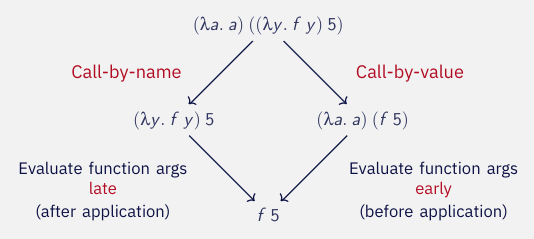
\includegraphics[width=0.75\linewidth]{images/call-by.png}
    \caption{There are often many different ways to reduce the same expression}
\end{figure}

The Church-Rosser Theorem states that if a term $t$ $\beta$-reduces to two terms $a$ and $b$, then there is a common term $t'$ to which both $a$ and $b$ are $\beta$-reducible.

\subsubsection{Equivalence}\label{equivalence}
The notion of \hyperref[confluence]{confluence} means we can define another notion of equivalence which equates more than \hyperref[alpha-equivalence]{$\alpha$-equivalence}.

Two terms are $\alpha\beta$-equivalent - written $\equiv_{\alpha\beta}$ - if they \hyperref[beta-reduction]{$\beta$-reduce} to $\alpha$-equivalent terms.

Furthermore there is another kind of equation that cannot be proved from $\beta$-equivalence alone called $\eta$-reduction:
\[(\lambda x.\:f\:x) \mapsto_\eta f\]

Adding this reduction to the system preserves confluence (and therefore the uniqueness of \hyperref[normal-forms]{normal forms}), so we have a notion of $\alpha\beta\eta$-equivalence also.

\subsection{Normal Forms}\label{normal-forms}
A \hyperref[lambda-term]{$\lambda$-term} which cannot be \hyperref[beta-reduction]{reduced} further is called a normal form.

Not every term has a normal form. Thankfully, all terms that do have a normal form are unique due to the \hyperref[church-rosser]{Church-Rosser theorem}.

This example reduces to itself:
$(\lambda x.\:x\:x)(\lambda x.\:x\:x)$

\subsection{Church Encodings}\label{church-encoding}
In order to demonstrate that \hyperref[lambda-calculus]{$\lambda$-calculus} is a usable programming language we need to show how to encode certain useful structures and primitives like booleans and natural numbers with their operations as \hyperref[lambda-term]{$\lambda$-terms}.

The general idea is to turn a data type into the type of its eliminator, in other words we make a function which serves the same purpose as the data type when used.

\subsubsection{Booleans}
We use booleans to choose between results, so the \hyperref[church-encoding]{encoding} of a boolean is a function that given two arguments returns the first if true and the second if false.

\[\text{True} \equiv \lambda a. \: \lambda b. \: a\]
\[\text{False} \equiv \lambda a. \: \lambda b. \: b\]

An If statement becomes:
\[\text{If} \equiv \lambda c. \: \lambda t. \: \lambda e. \: c\:t\:e\]

\subsubsection{Church Numerals}\label{church-numeral}
We use natural numbers to repeat processes $n$ times, so the \hyperref[church-encoding]{encoding} of a natural number is a function that takes a function $f$ and a value $x$ and will apply $f$ to $x$ that number of times.

\begin{equation}
\begin{aligned}
    \text{Zero} &\equiv \lambda f. \: \lambda x. \: x \nonumber \\
    \text{One}  &\equiv \lambda f. \: \lambda x. \: f \: x \nonumber \\
    \text{Two}  &\equiv \lambda f. \: \lambda x. \: f \: (f \: x) \nonumber \\
                &\;\;\vdots
\end{aligned}
\end{equation}

Then operations like the successor and addition are relatively simple:
\begin{equation}
\begin{aligned}
    \text{Suc} &\equiv \lambda n. \: \lambda f. \: \lambda x. \: f \: (n\:f\:x) \nonumber \\
    \text{Add}  &\equiv \lambda m. \: \lambda n. \: \lambda f. \: \lambda x. \: m \: f \: (n \: f \: x) \nonumber
\end{aligned}
\end{equation}

\subsection{The $\mathcal{Y}$ Combinator}\label{y-combinator}
The $\mathcal{Y}$ combinator is a "fixed point combinator", and it's the way we achieve recursion in \hyperref[lambda-calculus]{$\lambda$-calculus}. One $\mathcal{Y}$ combinator is the following:
\[\mathcal{Y} \equiv (\lambda f. \: (\lambda x. \: f \: (x \: x)) \: (\lambda x. \: f \: (x \: x)))\]


\subsection{Simply Typed $\lambda$-Calculus}
\subsubsection{Higher-Order Logic}
Originally the \hyperref[lambda-calculus]{$\lambda$-calculus} was intended for use as a term language for a logic, called higher-order logic.

The existence of the \hyperref[y-combinator]{$\mathcal{Y}$ combinator} and recursion in general causes a problem for this because we can cause statements like:
\[\mathcal{Y} \: \neg \equiv_\beta \neg \: (\mathcal{Y} \: \neg)\]

A logic which can have statements equivalent to their own negation is not ideal at all. To solve this church introduced \hyperref[types]{types}.

\subsubsection{Types}\label{types}
Typed \hyperref[lambda-calculus]{$\lambda$-calculus} has a set of base types like \texttt{nat} and \texttt{bool}.

Given two types $\sigma$ and $\tau$, $\sigma \to \tau$ is the type signature of a function from $\sigma$ to $\tau$, type signatures are right associative:
\[\sigma \to \tau \to \rho = \sigma \to (\tau \to \rho)\]

\hyperref[lambda-abstraction]{$\lambda$-abstraction} also specifies the type of the parameter: $\lambda x : \tau.\:t$

Things like the \hyperref[y-combinator]{$\mathcal{Y}$ combinator} or other recursive structures (things like the term which \hyperref[beta-reduction]{$\beta$-reduces} to itself) cannot be typed.


\subsubsection{Natural Deduction}
We can specify a logical system as a deductive system by providing a set of rules and axioms that describe how to prove various connectives. The same can be done for \hyperref[types]{typing}.

\[\frac{x : \tau \in \Gamma}{\Gamma \vdash t \: u : \tau}A \quad \frac{x : \sigma, \Gamma \vdash t : \tau}{\Gamma \vdash (\lambda x : \sigma.\:t) : \sigma \to \tau}I\]
\[\frac{\Gamma \vdash t : \sigma \to \tau \quad \Gamma \vdash u : \sigma}{\Gamma \vdash t \: u : \tau}E\]

This is the full rule-set for simply typed $\lambda$-calculus. The structure is that from the bottom you can derive the top, and that the right of the $\vdash$ symbol can be assumed true as a result of the left of it.

$A$ is assignment, $I$ is introduction, and $E$ is elimination.

\subsubsection{The Results of Simply Typed $\lambda$-calculus}
This \hyperref[types]{simply typed} \hyperref[lambda-calculus]{$\lambda$-calculus} has the following properties:
\begin{itemize}
    \item Uniqueness of types: In a given context (types for \hyperref[free-variables]{free variables}), any simply typed \hyperref[lambda-term]{$\lambda$-terms} has at most one type. Deciding this is in \hyperref[P]{\textbf{P}}.
    \item Subject reduction (or type safety): Typing respects \hyperref[equivalence]{$\equiv_{\alpha\beta\eta}$}, i.e. reduction does not affect a term's type.
    \item Strong normalisation: Any well-typed term evaluates in finitely many reductions to a unique irreducible term. If the type is a base type, this term is a constant.
\end{itemize}

The \hyperref[y-combinator]{$\mathcal{Y}$ combinator} cannot be typed, and strong normalisation means that such a term cannot exist.

If we want to do general computation in $\lambda$-calculus we need recursion back. The way this is done is by extending it to include a new built in feature called \textbf{fix}.

We extend $\beta$-reduction to unroll recursion in a single step (which will keep strong normalisation). 

Some type-theoretic languages avoid adding general recursion to the underlying $\lambda$-calculus - for reasons which are not examinable.

\newpage
\section{Definitions}
\subsection{Ambiguity}\label{ambiguity}
A grammar is \textbf{ambiguous} if there is more than one valid parse tree for a given string. This can cause problems with parsing and interpretation.


\subsection{Bijectivity}\label{bijection}
A \hyperref[binary-relation]{binary relation} $a \sim b$ is \textbf{bijective} if it is both \hyperref[injective]{injective} and \hyperref[surjective]{surjective}.


\subsection{Binary Relations}\label{binary-relation}
A \textbf{binary relation} associates elements of one set with elements of another, $a \sim b$ says that $a$ is related to $b$.

Relations are "one-to-many", meaning that $a$ can relate to more than one value.

Examples of a binary relations between numbers are $=$, $<$, and $\geq$.


\subsection{Closure}\label{closure}
A set $S$ is \textbf{closed} under an operation if that operation performed on elements of $S$ always produces another valid element of $S$.

The natural numbers are closed under addition, as adding two natural numbers together always produces a natural number.

They are not closed under subtraction however, as the result of $a - b$ when $b > a$ is not a natural number.


\subsubsection{Angelic and Demonic Non-determinism}\label{angel-devil}
A machine with \textbf{angelic} non-determinism accepts if at least one non-deterministic path reaches an accepting state. Angelic non-determinism is sometimes represented using $\exists$.

A machine with \textbf{demonic} non-determinism accepts only if every non-deterministic path reaches an accepting state. Demonic non-determinism is sometimes represented using $\forall$.


\subsection{Conjunctive Normal Form}\label{cnf}
A clause $\phi$ is in conjunctive normal form if it is of the form:
\[\bigwedge_i \bigvee_j P_{ij}\]

Where $P_{ij}$ is a literal (either a variable $P$ or a negation of one $\neg P$.

$\phi$ is in $k$-CNF if each clause $\bigvee P_{ij}$ has at most $k$ literals.


\subsection{Computable Functions}\label{computable}
A \hyperref[total]{total function} $\mathbb{N} \to \mathbb{N}$ is \textbf{computable} if there is a \hyperref[rm]{RM}/\hyperref[tm]{TM} which computes $f$, i.e. given an $x$ in $R_0$ leaves $f(x)$ in $R_0$.


\subsection{Decidability}\label{decidable}
A \hyperref[decision problem]{decision problem} $(D, Q)$ is decidable or \hyperref[computable]{computable} if $d \in Q$ is characterised by a computable function $f : D \to \{0, 1\}$.

A problem which is both semi-decidable and co-semi-decidable is decidable. There are problems which are neither semi-decidable or co-semi-decidable.

\subsubsection{Semi-decidability}\label{semi-decidable}
The \hyperref[halting]{halting problem} is not symmetric. If $M \in H$ we can determine this: run $M$ - when it halts it will say "yes". But, if $M \not \in H$ we can't determine this by running $M$ as it will run forever. The halting problem is semi-decidable.

A \hyperref[decision problem]{decision problem} $(D, Q)$ is semi-decidable if there is a \hyperref[rm]{RM}/\hyperref[tm]{TM} that returns "yes" for every $d \in Q$ but may return "no" or loop forever when $d \not \in Q$.

If a problem $P$ is semi-decidable, its complement $\overline P$ is co-semi-decidable.

Semi-decidable problems are sometimes called recognisable.

\subsubsection{Co-semi-decidability}\label{co-semi-decidable}
The \hyperref[looping]{looping problem} is not symmetric. If $M \not \in L$ we can determine this: run $M$ - when it halts it will say "no". But, if $M \in L$ we can't determine this by running $M$ as it will run forever. The looping problem is co-semi-decidable.

A \hyperref[decision problem]{decision problem} $(D, Q)$ is co-semi-decidable if there is a \hyperref[rm]{RM}/\hyperref[tm]{TM} that returns "no" for every $d \not \in Q$ but may return "yes" or loop forever when $d \in Q$.

If a problem $P$ is co-semi-decidable, its complement $\overline P$ is semi-decidable.


\subsection{Decision Problems}\label{decision-problem}
A decision problem is a set $D$ and a query subset $Q \subseteq D$. Decision problems can be \hyperref[decidable]{decidable}, \hyperref[semi-decidable]{semi-decidable}, or \hyperref[co-semi-decidable]{co-semi-decidable}.

In language problems (\hyperref[dfa]{DFAs} and \hyperref[cfg]{CFGs} etc.) are decision problems where $D = \Sigma^*$ and $Q$ is the language in question.

Other such problems are $D = \mathbb{N}$ and $Q =$ Primes, or $D=$ RMs and $Q =$ halting RMs

Decidable languages are closed under union, intersection, and complement


\subsection{Determinism and Non-determinism}\label{deterministic}
A function $f : A \to B$ is \textbf{deterministic} if when given a particular input in $A$, will always produce the same output from $B$.

A function $f : A \to B$ is \textbf{non-deterministic} if when given a particular input in $A$ doesn't always produce the same output from $B$.


\subsection{Enumerable}\label{enumerable}
A set $S$ is \textbf{enumerable} if there is a \hyperref[bijection]{bijection} between $S$ and $\mathbb{N}$.


\subsection{Equivalence Classes}\label{equivalence-class}
An \textbf{equivalence class} of a set $S$ is some subset of $S$ such that every element of $S$ has an \hyperref[equivalence-relation]{equivalence relation} to every other element of $S$.

Every element of $S$ is contained in exactly one equivalence class, though it may be the only element in that class.


\subsection{Equivalence Relations}\label{equivalence-relation}
A binary relation $a \sim b$ is an \textbf{equivalence relation} if it is \hyperref[reflexive]{reflexive}, \hyperref[symmetric]{symmetric}, and \hyperref[transitive]{transitive}.

Equality $(=)$ is an equivalence relation because it can be shown to be reflexive, symmetric, and transitive. Having the same birthday is an equivalence relation on the set of birthdays.


\subsection{Injectivity}\label{injective}
A \hyperref[binary-relation]{binary relation} $a \sim b$ is \textbf{injective} if every element in the domain maps to one unique element of the range, injective functions are "one-to-one" mappings.


\subsection{Interleaving}\label{interleaving}
The set of valid \hyperref[rm]{RM} descriptions is decidable, given $n \in \mathbb{N}$ we can check whether $n = \ulcorner M \urcorner$ for some machine $M$.

This means we can sequentially enumerate all machines $\ulcorner M_0 \urcorner, \ulcorner M_1 \urcorner, \dots$

Interleaving is the process of running all register machines in sequence one step at a time, and checking some \hyperref[decision-problem]{decision problem} as we go.\\

\begin{lstlisting}[language=Python]
ms = $\langle \rangle$; i = 0;

while true {
    ms = ms ++ $\langle \ulcorner M_i \urcorner \rangle$;
    for $\ulcorner M \urcorner$ in ms {
        run $M$ for one step, and update ms;
        if [[condition]] is met {
            output $\ulcorner M \urcorner$;
            delete $M$ from ms;
        }
    }
}

\end{lstlisting}


\subsection{Kleene Star}\label{kleene-star}
The \textbf{Kleene closure} of a language $L$ - written $L^*$ - is the language of strings that consist wholly of zero or more strings in $L$
\[L^*=\bigcup_{i \in \mathbb{N}} L^i\]

Regular languages are \hyperref[closure]{closed} under Kleene Closure


\subsection{Machine Properties}\label{property}
A property is a set of \hyperref[rm]{RM}/\hyperref[tm]{TM} descriptions

\subsubsection{Nontrivial Properties}\label{nontrivial}
A \hyperref[property]{property} is nontrivial if it contains some but not all descriptions.

Trivial properties hold for all languages or for none.

\subsubsection{Semantic Properties}\label{semantic}
A \hyperref[property]{property} $P$ is semantic if:
\[\mathcal{L}(M_1) = \mathcal{L}(M_2) \Rightarrow (\ulcorner M_1 \urcorner \in P \Leftrightarrow \ulcorner M_2 \urcorner \in P)\]

In other words, it concerns the language and not the particular implementation of the machine.


\subsection{Nondeterminism in RM and TM}\label{nrm}\label{ntm}
We can have nondeterministic \hyperref[rm]{RM} and \hyperref[tm]{TM} just as we can have \hyperref[nfa]{nondeterministic finite automata}.

For register machines this involves adding a special instruction \texttt{MAYBE(j)} which will either nondeterministically jump to to $I_j$ or do nothing.

An NRM accepts if there is some run (a sequence of instructions through the choices) that halts and accepts. The presence of infinite runs doesn't matter here because we only care about if there are accepting finite runs.

An NRM has the same deciding power as a regular RM, as we can use \hyperref[interleaving]{interleaving} to simulate all runs of an NRM at once on a regular RM - however, in time $n$ an RM can only explore $\mathcal{O}(n)$ possibilities where an NRM can explore $2^{\mathcal{O}(n)}$ possibilities.

All of the above is true of NTMs, with some minor differences to get the same results.


\subsection{Oracles}\label{oracle}
Given a \hyperref[decision-problem]{decision problem} $(D, Q)$, an \textbf{oracle} for $Q$ is a "magic" \hyperref[rm]{RM} instruction \texttt{ORACLE}$_Q(i)$ which, given an encoding of $d \in D$ in $R_i$ sets $R_i$ to contain $1$ iff $d \in Q$.

An oracle is only useful when it predicts for an \hyperref[undecidable]{undecidable} problem, as an oracle for a \hyperref[decidable]{decidable} problem could be replaced by a a program which decidably computes that result.


\subsection{Pairing Functions}\label{pairing-function}
A \textbf{pairing function} is an \hyperref[injective]{injective} function $\mathbb{N} \times \mathbb{N} \to \mathbb{N}$.

An example is $f(x, y) = 2^x3^y$

We write $\langle x, y \rangle_2$ to denote the result of pairing two values $x$ and $y$. If $z = \langle x, y \rangle_2$ then we say $z_0 = x$ and $z_1 = y$.

A function which pairs two numbers is enough to generalise to cram an arbitrarily long sequence of numbers into one.


\subsection{Parse Trees}\label{parse-trees}
A parse tree is a tree that shows how to devise a string of characters from a non-terminal state of a \hyperref[cfg]{CFG}.

\begin{figure}[H]
    \centering
    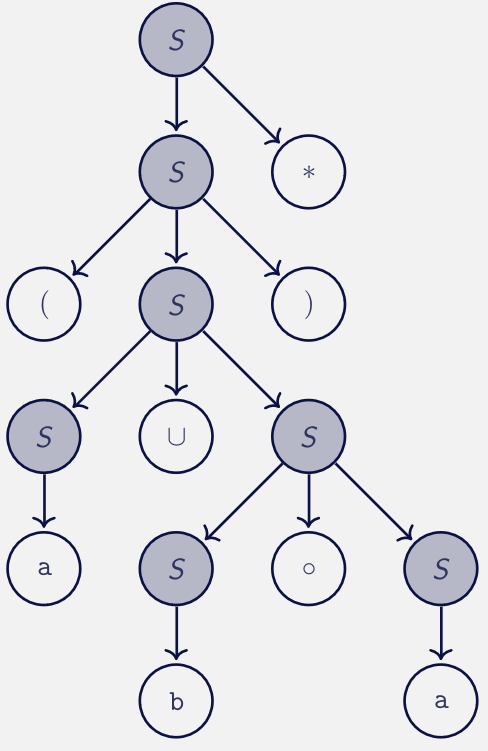
\includegraphics[width=0.35\linewidth]{images/parse-tree.png}
    \caption{The yield of this tree is $(a \cup b^*) \circ a$}
\end{figure}

The yield of a parse tree is the concatenation of all the symbols at its leaves. If the route of the tree is $S$ then the yield $x \in \mathcal{L}(G)$.

Parse trees are typically left-associative, meaning that we parse assuming that left bracketing is correct.


\subsection{Pigeonhole Principle}\label{pigeonhole-principle}
The \textbf{pigeonhole principle} states that if you have $n$ items are put into $m$ containers, where $n > m$, at least one of the containers must have more than one item in it.


\subsection{Power Set}\label{power-set}
The \textbf{power set} of a given set $S$, denoted $\mathcal{L}(S)$ is the set containing all subsets of $S$, including $\emptyset$ and $S$ itself.

\[\mathcal{P}(S) = \{s \:|\: s \subseteq S\}\]

Given $n=|S|$, $|\mathcal{P}(S)|=2^n$.


\subsection{Reflexivity}\label{reflexive}
A binary relation is \textbf{reflexive} if every value relates to itself, i.e. $a \sim a$.

Equality $(=)$ is a reflexive binary relation between two numbers, where strictly less than $(<)$ is not - because $a < a$ isn't true.


\subsection{Satisfiability}
\subsubsection{SAT}\label{sat}
SAT is a \hyperref[decision-problem]{decision problem} which asks the following question: given a boolean formula $\phi$ over a set of boolean variables $X_i$, is there an assignment of values to $X_i$ which satisfies $\phi$?

\[(A \vee B) \wedge (\neg B \vee C) \wedge (A \vee C)\text{ is satisfiable by making $A, C = \top$}\]

The size of a SAT problem is the number of symbols in $\phi$.

\subsubsection{3SAT}
3SAT is the problem of determining \hyperref[sat]{satisfiability} for formula given in \hyperref[cnf]{3-CNF}.


\subsection{Sequential Composition}\label{sequential-composition}
The \textbf{sequential composition} of two languages $L_1$ and $L_2$ - written $L_1L_2$ - is the language of strings that consist of a string in $L_1$ followed by a string in $L_2$.

\[ L_1L_2=\{vw | v \in L_1, w \in L_2\} \]

Regular languages are closed under sequential composition.


\subsection{Surjectivity}\label{surjective}
A \hyperref[binary-relation]{binary relation} $a \sim b$ is \textbf{surjective} if every element $b$ in the co-domain $B$ is mapped to by at least one element $a$ in the domain $A$.


\subsection{Symmetry}\label{symmetric}
A binary relation is \textbf{symmetric} if $a \sim b \Leftrightarrow b \sim a$.

Equality $(=)$ is symmetric, as $a = b$ means $b = a$. Greater than or equal $(\geq)$ is not symmetric, as $a \geq b$ doesn't necessarily mean $b \geq a$.


\subsection{Time Complexity}\label{time-complexity}
The time complexity of a deterministic machine $M$ that halts on all inputs is a function $f : \mathbb{N} \to \mathbb{N}$ where $f(n)$ is the maximum number of steps that $M$ uses on any input of size $n$.

\subsubsection{Big $\mathcal{O}$}
Let $f, g : \mathbb{N} \to \mathbb{R}_{\geq 0}$. Say that $f(n) \in \mathcal{O}(g(n))$ if there exists $c, n_0 > 0$ such that for all $n > n_0$: 
\[f(n) \leq c \cdot g(n)\]

\subsubsection{Big $\Omega$}
Let $f, g : \mathbb{N} \to \mathbb{R}_{\geq 0}$. Say that $f(n) \in \Omega(g(n))$ if there exists $c, n_0 > 0$ such that for all $n > n_0$:
\[f(n) \geq c \cdot g(n)\]


\subsection{Total and Partial Functions}\label{total-partial}
A \textbf{total} function $f : A \to B$ is a function which is defined for every input value in $A$.

A \textbf{partial} function $f : A \rightharpoonup B$ is a function which may not be defined on every input value in $A$, it returns either an element of $B$ or $\bot$.


\subsection{Transitivity}\label{transitive}
A binary relation is \textbf{transitive} if when $a \sim b$ and $b \sim c$, $a \sim c$.

Equality $(=)$ is transitive, because if $a = b$ and $b = c$ we know $a = c$. Strictly less than $(<)$ is also transitive, as if $a < b$ and $b < c$, we know $a < c$.


\subsection{Turing Machines}\label{tm}
A turing machine is a 7-tuple $(Q, \Sigma, \Gamma, \delta, q_0, q_{accept}, q_{reject})$:
\begin{itemize}
    \item $Q:$ states
    \item $\Sigma:$ input symbols
    \item $\Gamma \supseteq \Sigma:$ tape symbols, including a blank symbol $\textvisiblespace$
    \item $\delta: Q \times \Gamma \to Q \times \Gamma \times \{-1, +1\}:$ a transition function
    \item $q_0, q_{accept}, q_{reject} \in Q:$ start, accept, and reject states
\end{itemize}

Turing machines are \hyperref[church-turing]{equivalent in power} to \hyperref[rm]{register machines}, the proof of which involves creating an RM to simulate a TM, and vice versa.

The upshot of this equivalence is that the halting problem applies to TMs just as with RMs.

None of the following adds any extra expressively: the ability to stay in place, making the tape unbounded in both directions, restricting the number of symbols, having multiple tapes, and adding non-determinism.


\subsection{Turing Transducers}\label{turing-transducer}
A \textbf{Turing Transducer} is a \hyperref[rm]{RM}/\hyperref[tm]{TM} which takes an instance $d$ of a problem $P_1 = (D_1, Q_1)$ in $R_0$ and halts with an instance $d' = f(d)$ of $P_2 = (D_2, Q_2)$ in $R_0$. Thus, $f$ is a computable function $D_1 \to D_2$.


\subsection{Undecidable Problems}\label{undecidable-problems}
\subsubsection{$A$}
\[A = \{\langle \ulcorner M \urcorner, w \rangle \:|\: M \text{ accepts } w\}\]

This is analogous to the proof for the \hyperref[halting]{halting problem}.

\subsubsection{$NotEmpty$}
\[NotEmpty = \{\ulcorner M \urcorner \:|\: \mathcal{L}(M) \neq \emptyset\}\]

We can sketch a \hyperref[mapping-reduction]{mapping reduction} from $A$. Given an instance $\langle M, w \rangle$ of $A$, our reduction constructs a machine $M'$ whose language is either $\{w\}$ or $\emptyset$.

Given input $x$, it will reject if $x \neq w$, else run $M$ on $w$. We know that $\langle M, w \rangle \in A$ iff $M' \in NotEmpty$ too is undecidable.

\subsubsection{Uniform Halting: $UH$}
\[UH = \{\ulcorner M \urcorner \:|\: M \text{ halts on all inputs}\}\]

This is a demonic version of the halting problem. We can reduce from $H$ to $UH$. Given a machine $M$ and an input $w$, build a machine $M'$ which ignores its input, writes $w$ to the tape, and then behaves as $M$. Then $M'$ halts on any inut iff $M$ halts on $w$.

\subsubsection{The Looping Problem: $L$}\label{looping}
Let $L$ be the subset of \hyperref[rm]{RMs}/\hyperref[tm]{TMs} that go into an infinite loop.

Since $L$ is the complement of \hyperref[halting]{$H$} this seems easy, but we can't fit it neatly into our definition of a \hyperref[mapping-reduction]{mapping reduction}.

However, since $L$ is \hyperref[turing-reduction]{Turing reducible} to $H$ we can show it is \hyperref[undecidable]{undecidable}.

\end{document}
